
%==============================================================================
\section{Adaptive Linear Threshold for Encrypted Comparison}
\label{sec:alt_method}
%==============================================================================

\subsection{Problem Statement}

Standard CKKS supports addition and multiplication but \emph{not} comparison. Given $E(x)$ and threshold $T$, determining whether $x > T$ without decryption is fundamentally challenging because HE schemes operate on algebraic structures that lack natural ordering. Existing approaches~\cite{Kim2018comparison, Cheon2019comparison} require deep polynomial circuits (depth 8--15), consuming significant noise budget.

\subsection{Our Solution: Adaptive Linear Threshold (ALT)}

\noindent\textbf{Key Insight:} For load balancing decisions, we need only a \emph{soft indicator}---not an exact binary decision. We approximate the step function with a single linear function:

\begin{equation}
    S(x, T, k) = 0.5 + \frac{x - T}{2\delta} = \underbrace{\left(0.5 - \frac{T}{2\delta}\right)}_{\text{intercept } b} + \underbrace{\frac{1}{2\delta}}_{\text{slope } a} \cdot x
    \label{eq:alt}
\end{equation}
where $\delta = T/k$ is the soft-zone half-width and $k$ is the sensitivity parameter. The encrypted computation requires only:
\begin{equation}
    E(S) = E(x) \times a + b \quad \text{(one \texttt{multiply\_plain} + one \texttt{add\_plain})}
\end{equation}

\noindent\textbf{This has multiplicative depth \textbf{zero}}---no ciphertext--ciphertext multiplication is required.

\subsection{Mathematical Properties}

\begin{table}[H]
\centering
\caption{ALT Score Properties}
\label{tab:alt_properties}
\begin{tabular}{@{}lll@{}}
\toprule
\textbf{Input value $x$} & \textbf{Score $S(x)$} & \textbf{Interpretation} \\
\midrule
$x = T - \delta$ & $S = 0.0$ & Definitely below \\
$x = T$ & $S = 0.5$ & At threshold (uncertain) \\
$x = T + \delta$ & $S = 1.0$ & Definitely above \\
$x \ll T$ & $S < 0$ (clamped to 0) & Far below \\
$x \gg T$ & $S > 1$ (clamped to 1) & Far above \\
\bottomrule
\end{tabular}
\end{table}

\subsection{Confidence Zone Classification}

After decryption by the utility, the score is classified:
\begin{equation}
    \texttt{Zone}(S) = \begin{cases}
        \texttt{BELOW} & \text{if } S < 0.3, \quad \text{confidence} = 1 - S/0.3 \\
        \texttt{UNCERTAIN} & \text{if } 0.3 \leq S \leq 0.7 \\
        \texttt{ABOVE} & \text{if } S > 0.7, \quad \text{confidence} = (S - 0.7)/0.3
    \end{cases}
\end{equation}

\subsection{Adaptive Sensitivity}

The sensitivity $k$ is computed adaptively based on the expected value range $(x_{\min}, x_{\max})$:
\begin{equation}
    k = \min\left(15, \max\left(3, \frac{5}{\max(0.1, \; \text{edge\_factor})}\right)\right)
\end{equation}
where $\text{edge\_factor} = \min\left(\frac{T - x_{\min}}{x_{\max} - x_{\min}}, \; 1 - \frac{T - x_{\min}}{x_{\max} - x_{\min}}\right)$.

\subsection{Comparison with Polynomial Methods}

\begin{table}[H]
\centering
\caption{ALT vs.\ Polynomial Comparison Methods}
\label{tab:alt_vs_poly}
\footnotesize
\begin{tabular}{@{}lccc@{}}
\toprule
\textbf{Method} & \textbf{Depth} & \textbf{Prec.} & \textbf{Type} \\
\midrule
Minimax~\cite{Kim2018comparison} & 8--12 & High & Hard \\
Composite~\cite{Cheon2019comparison} & 10--15 & V.~High & Hard \\
Chebyshev~\cite{Iliashenko2021} & 6--10 & High & Hard \\
\textbf{ALT (ours)} & \textbf{0} & Soft & \textbf{Soft} \\
\bottomrule
\end{tabular}
\end{table}

\begin{figure}[H]
    \centering
    
\includegraphics[width=\columnwidth]{fig_alt_threshold.png}
    \caption{Adaptive Linear Threshold score for $T = 100$ kW, $k = 7$. The uncertain zone $[85.7, 114.3]$ kW spans $\pm 14.3\%$ around the threshold.}
    \label{fig:alt_threshold}
\end{figure}

%==============================================================================
\section{Verifiable Aggregation Protocol}
\label{sec:verification}
%==============================================================================

\subsection{Motivation}

A malicious coordinator could compute an incorrect aggregate (inflating or deflating the total demand), causing inappropriate load balancing decisions. We integrate Pedersen commitments~\cite{Pedersen1991} alongside CKKS encryption.

\subsection{Protocol Description}

\noindent\textbf{Step 1 (Agent):} Each agent $i$ creates:
\begin{align}
    E(\mathbf{d}_i) &= \texttt{CKKS.Encrypt}(\mathbf{d}_i, \text{pk}) \\
    C_i &= g^{d_i \cdot s} \cdot h^{r_i} \bmod p \\
    O_i &= (d_i, r_i) \quad \text{(opening, kept secret)}
\end{align}

\noindent\textbf{Step 2 (Coordinator):} Aggregates FHE and commitments:
\begin{align}
    E\left(\sum d_i\right) &= \sum E(\mathbf{d}_i) \\
    C_{\text{agg}} &= \prod_{i=1}^{n} C_i = g^{(\sum d_i) \cdot s} \cdot h^{\sum r_i} \bmod p
\end{align}

\noindent\textbf{Step 3 (Utility):} Decrypts and verifies:
\begin{equation}
    \hat{D} = \texttt{Decrypt}\left(E\left(\sum d_i\right)\right), \quad C_{\text{agg}} \stackrel{?}{=} g^{\hat{D} \cdot s} \cdot h^{\sum r_i} \bmod p
\end{equation}

\begin{figure}[H]
    \centering
    \includegraphics[width=\columnwidth]{aggregation.png}
    \caption{Verifiable aggregation protocol flow. Each household agent sends encrypted demand $E(\mathbf{d}_i)$ and Pedersen commitment $C_i$ to the coordinator, and openings $(d_i, r_i)$ to the utility via a secure channel. The coordinator aggregates both FHE values and commitments, and the utility verifies integrity by checking commitment consistency after decryption.}
    \label{fig:aggregation}
\end{figure}

\subsection{Security Properties}

\begin{table}[H]
\centering
\caption{Verifiable Aggregation Security Properties}
\label{tab:ver_security}
\footnotesize
\begin{tabular}{@{}lp{5.5cm}@{}}
\toprule
\textbf{Property} & \textbf{Guarantee} \\
\midrule
Hiding & Reveals nothing about $d_i$ (info.-theoretic) \\
Binding & Cannot open to $d_i' \neq d_i$ (DL hard) \\
Soundness & Cheating detected w.p.\ 1 \\
Non-interact. & Single-round, no interactive proofs \\
\bottomrule
\end{tabular}
\end{table}

\subsection{Pedersen Commitment Parameters}

\begin{table}[H]
\centering
\caption{Pedersen Commitment Configuration}
\label{tab:pedersen_params}
\footnotesize
\begin{tabular}{@{}lp{2cm}p{3cm}@{}}
\toprule
\textbf{Param.} & \textbf{Value} & \textbf{Source} \\
\midrule
Prime $p$ & 2048-bit & RFC~3526 Group~14 \\
Generator $g$ & 2 & Standard choice \\
Generator $h$ & $g^{\text{SHA256}}$ & Nothing-up-my-sleeve \\
Scale $s$ & $10^6$ & 6 decimal places \\
Group order & $p - 1$ & Mult.\ group \\
\bottomrule
\end{tabular}
\end{table}

%==============================================================================
\section{Noise and Depth Analysis}
\label{sec:noise}
%==============================================================================

\subsection{Automatic Parameter Selection}

Our system implements depth-adaptive parameter configuration (Algorithm~\ref{alg:param_select}). Given a requested multiplicative depth $d$:

\begin{algorithm}[htbp]
\caption{Automatic FHE Parameter Selection}
\label{alg:param_select}
\begin{algorithmic}[1]
\REQUIRE Requested multiplicative depth $d$
\ENSURE CKKS parameters $(N, \mathbf{q}, \Delta)$
\STATE $N \leftarrow 16384$ \textbf{if} $d \leq 8$ \textbf{else} $32768$
\STATE $B_{\max} \leftarrow 438$ \textbf{if} $N = 16384$ \textbf{else} $881$
\STATE $B_{\text{edge}} \leftarrow 50$; \quad $B_{\text{avail}} \leftarrow B_{\max} - 2 B_{\text{edge}}$
\STATE $B_{\text{mid}} \leftarrow \min(40, \lfloor B_{\text{avail}} / d \rfloor)$
\IF{$B_{\text{mid}} < 30$}
    \STATE \textbf{raise} ``Depth exceeds leveled CKKS limits''
\ENDIF
\STATE $\mathbf{q} \leftarrow [B_{\text{edge}}, \underbrace{B_{\text{mid}}, \ldots, B_{\text{mid}}}_{d}, B_{\text{edge}}]$
\STATE $\Delta \leftarrow 2^{\max(20, \min(30, B_{\text{mid}} - 5))}$
\RETURN $(N, \mathbf{q}, \Delta)$
\end{algorithmic}
\end{algorithm}

\subsection{Configuration Examples}

\begin{table}[H]
\centering
\caption{Auto-Selected Parameters for Various Depths}
\label{tab:auto_params}
\footnotesize
\resizebox{\columnwidth}{!}{%
\begin{tabular}{@{}cccccc@{}}
\toprule
\textbf{Depth} & $N$ & \textbf{Chain} & \textbf{Bits} & $\Delta$ & \textbf{Status} \\
\midrule
2 & 16384 & [50,40,40,50] & 180 & $2^{30}$ & \ding{51} OK \\
5 & 16384 & [50,40$\times$5,50] & 300 & $2^{30}$ & \ding{51} OK \\
8 & 16384 & [50,40$\times$8,50] & 420 & $2^{30}$ & \ding{51} OK \\
10 & 32768 & [50,40$\times$10,50] & 500 & $2^{30}$ & \ding{51} OK \\
20 & 32768 & [50,39$\times$20,50] & 880 & $2^{30}$ & \ding{51} OK \\
25 & 32768 & [50,31$\times$25,50] & 875 & $2^{26}$ & \ding{51} Tight \\
\bottomrule
\end{tabular}}
\end{table}

\subsection{Noise Growth Characterization}

The stress test module measures decryption error after repeated ciphertext--ciphertext multiplications using initial value $v = 2.0$ and multiplier $\mu = 1.125$:
\begin{equation}
    E(v_k) = E(v_{k-1}) \otimes E(\mu), \quad v_k^{\text{expected}} = v_0 \cdot \mu^k
\end{equation}

\begin{equation}
    \epsilon_{\text{abs}}^{(k)} = |\hat{v}_k - v_k^{\text{expected}}|, \quad \epsilon_{\text{rel}}^{(k)} = \frac{\epsilon_{\text{abs}}^{(k)}}{\max(|v_k^{\text{expected}}|, 10^{-12})}
\end{equation}

\begin{figure}[H]
    \centering
    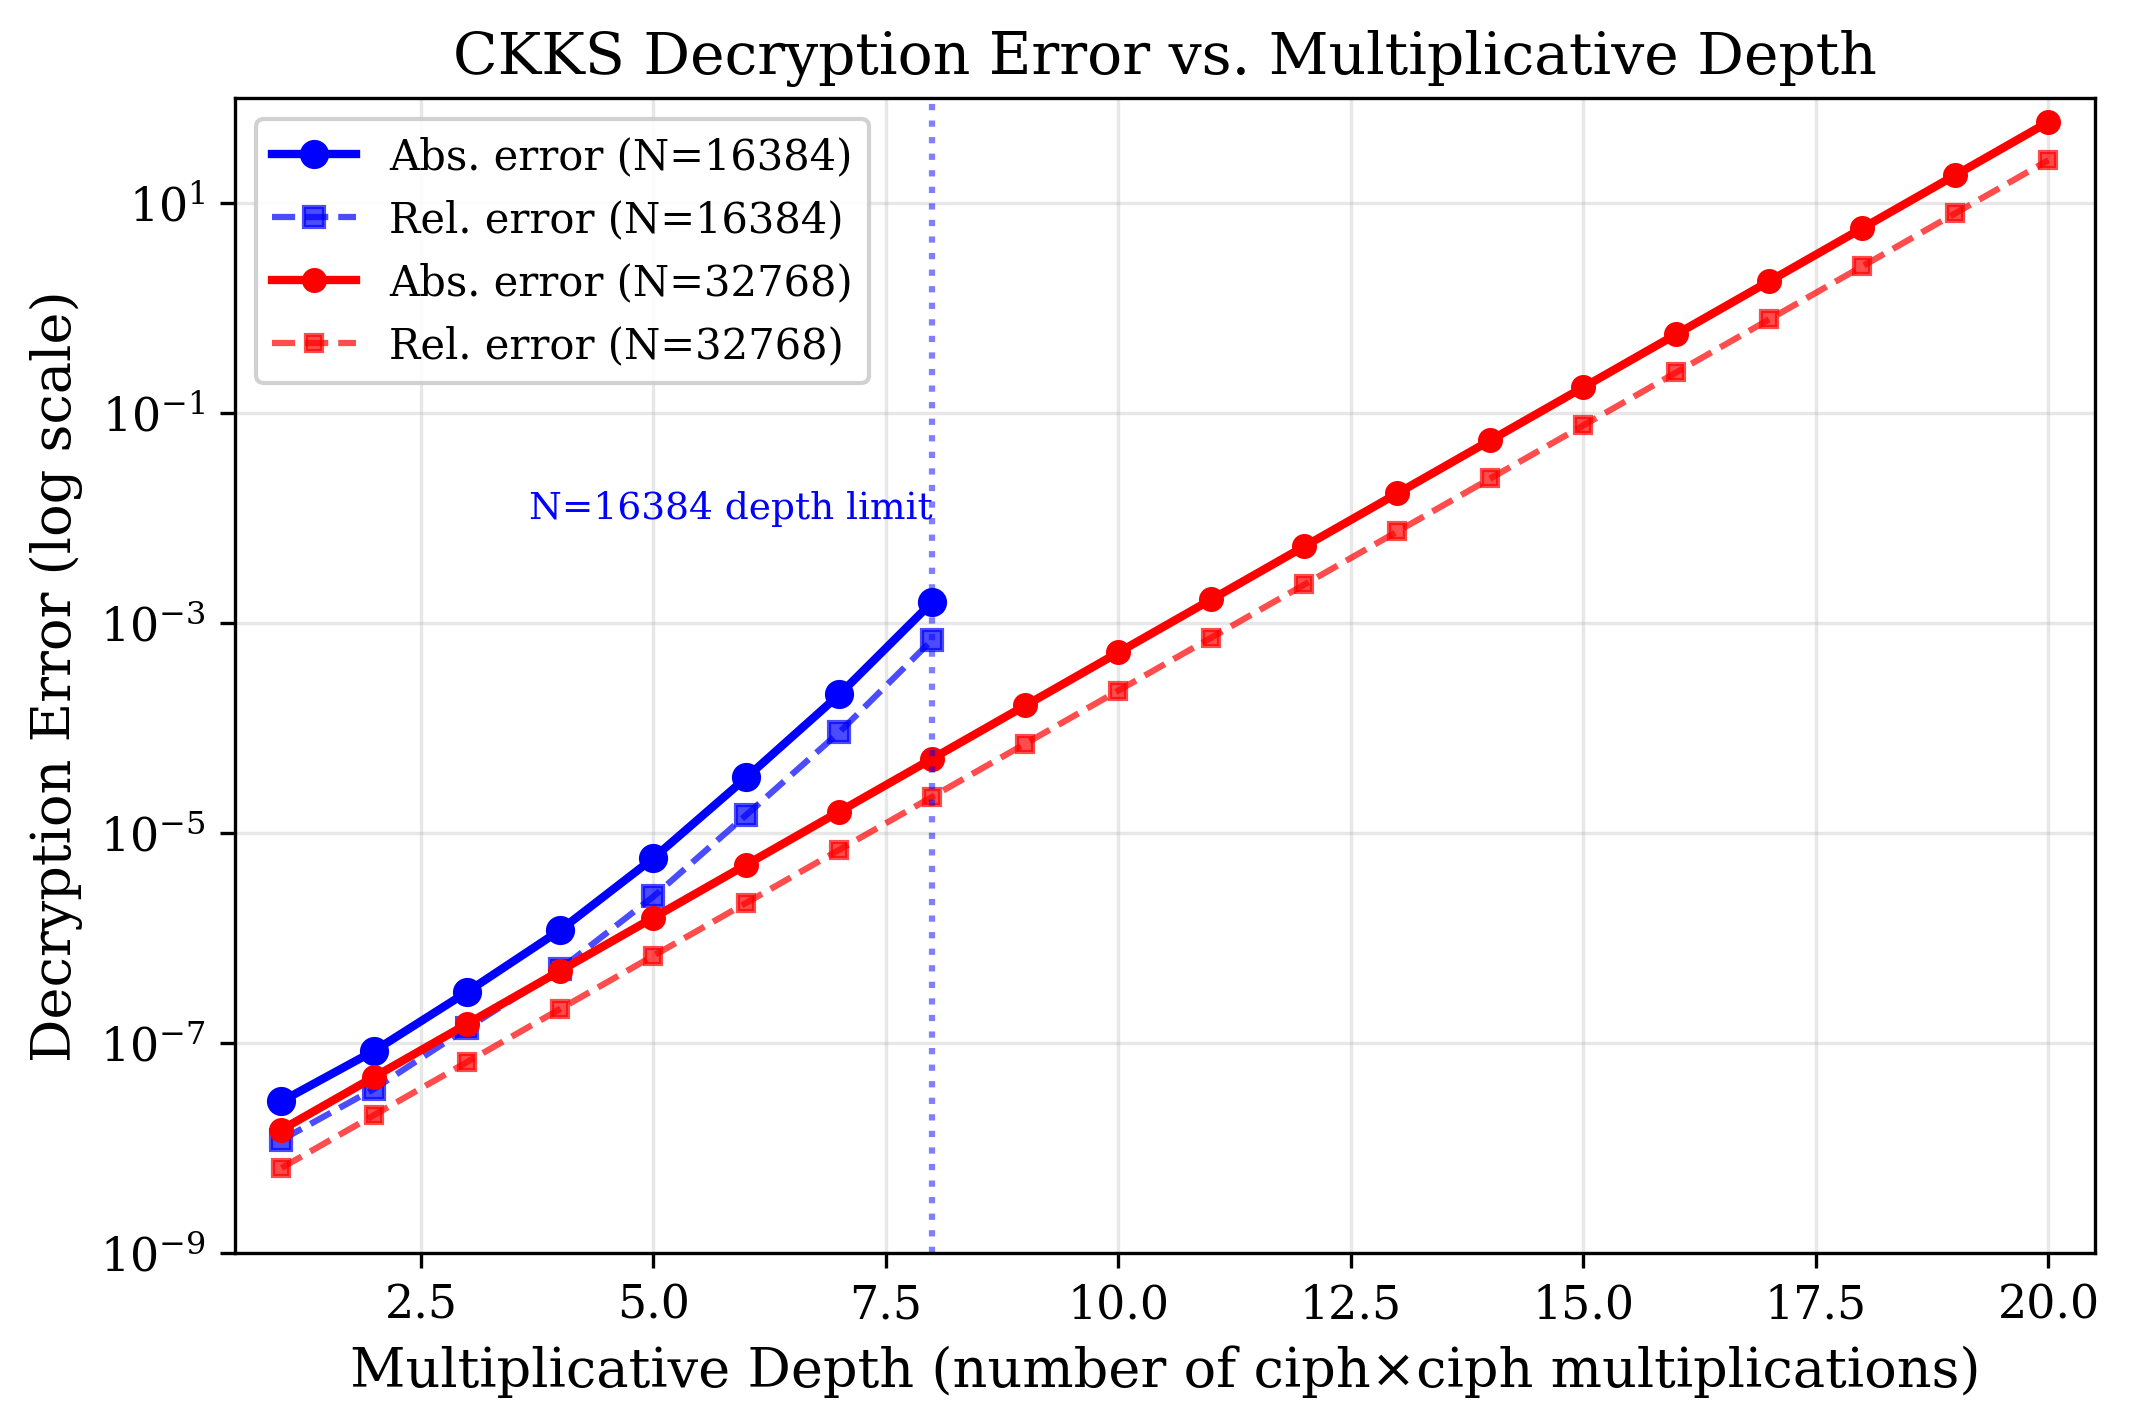
\includegraphics[width=\columnwidth]{fig_noise_depth.png}
    \caption{CKKS decryption error vs.\ multiplicative depth. Error grows exponentially with depth, with noise budget exhaustion causing failure beyond the scheme's configured maximum.}
    \label{fig:noise_depth}
\end{figure}

%==============================================================================
\section{Experimental Results}
\label{sec:results}
%==============================================================================

All experiments were conducted on a Windows 11 system with Python 3.10 and TenSEAL 0.3.x, using Intel Core i7 @ 2.8 GHz with 16 GB RAM.

\subsection{Runtime Performance Profiling}

\begin{table}[H]
\centering
\caption{Runtime Performance ($N{=}16384$, $\Delta{=}2^{40}$)}
\label{tab:performance}
\footnotesize
\resizebox{\columnwidth}{!}{%
\begin{tabular}{@{}lccccc@{}}
\toprule
\textbf{Operation} & \textbf{Dim} & \textbf{Enc.} & \textbf{Comp.} & \textbf{Dec.} & \textbf{Total} \\
 & & (ms) & (ms) & (ms) & (ms) \\
\midrule
$E(\mathbf{a}) \odot E(\mathbf{b})$ & 4 & 15 & 8 & 5 & 28 \\
$E(\mathbf{a}) \cdot E(\mathbf{b})$ & 4 & 15 & 12 & 5 & 32 \\
$E(\mathbf{a}) \times E(\mathbf{b})$ & 3 & 15 & 95 & 8 & 118 \\
$\mathbf{M} \cdot E(\mathbf{v})$ & 3$\times$3 & 15 & 30 & 15 & 60 \\
$E(\mathbf{M}) \cdot E(\mathbf{v})$ & 3$\times$3 & 60 & 45 & 15 & 120 \\
$E(\mathbf{M}) \cdot E(\mathbf{v})$ & 5$\times$5 & 90 & 85 & 25 & 200 \\
$E(\mathbf{M}) \cdot E(\mathbf{v})$ & 10$\times$10 & 165 & 195 & 50 & 410 \\
ALT threshold & 1 & 8 & 2 & 5 & 15 \\
Aggregation & 25 ag. & -- & 110 & 5 & 115 \\
Aggregation & 100 ag. & -- & 400 & 5 & 405 \\
\bottomrule
\end{tabular}}
\end{table}

\FloatBarrier
\subsection{Numerical Accuracy Verification}

\begin{table}[H]
\centering
\caption{Numerical Accuracy: Decrypted vs.\ Expected}
\label{tab:accuracy}
\footnotesize
\resizebox{\columnwidth}{!}{%
\begin{tabular}{@{}lcccc@{}}
\toprule
\textbf{Operation} & \textbf{Dim} & $\|\epsilon\|_2$ & $\|\epsilon\|_\infty$ & \textbf{Rel.\ Err.} \\
\midrule
Element-wise & 4 & $<10^{-6}$ & $<10^{-7}$ & $<10^{-7}$ \\
Dot product & 4 & $<10^{-6}$ & $<10^{-7}$ & $<10^{-7}$ \\
FHE Mat-Vec & 3$\times$3 & $<10^{-5}$ & $<10^{-6}$ & $<10^{-6}$ \\
Plain Mat-Vec & 3$\times$3 & $<10^{-6}$ & $<10^{-7}$ & $<10^{-7}$ \\
Cross product & 3 & $<10^{-3}$ & $<10^{-4}$ & $<10^{-4}$ \\
ALT ($T{=}100$) & 1 & $<10^{-6}$ & $<10^{-6}$ & $<10^{-7}$ \\
Aggregation & 25 & $<10^{-6}$ & $<10^{-7}$ & $<10^{-8}$ \\
\bottomrule
\end{tabular}}
\end{table}

\FloatBarrier
\subsection{Ciphertext Size Analysis}

\begin{table}[H]
\centering
\caption{Ciphertext Sizes and Communication Overhead}
\label{tab:ct_sizes}
\footnotesize
\resizebox{\columnwidth}{!}{%
\begin{tabular}{@{}lcccc@{}}
\toprule
\textbf{Operation} & \textbf{In CTs} & \textbf{In KB} & \textbf{Out CTs} & \textbf{Out KB} \\
\midrule
$E(\mathbf{a}) \odot E(\mathbf{b})$ & 2 & 262 & 1 & 131 \\
$E(\mathbf{a}) \cdot E(\mathbf{b})$ & 2 & 262 & 1 & 131 \\
$\mathbf{M}{\cdot}E(\mathbf{v})$ (3$\times$3) & 1 & 131 & 3 & 393 \\
$E(\mathbf{M}){\cdot}E(\mathbf{v})$ (3$\times$3) & 4 & 524 & 3 & 393 \\
$E(\mathbf{M}){\cdot}E(\mathbf{v})$ (10$\times$10) & 11 & 1441 & 10 & 1310 \\
$E(\mathbf{a}) \times E(\mathbf{b})$ (3D) & 2 & 262 & 1 & 131 \\
\bottomrule
\end{tabular}}
\end{table}

\begin{figure}[H]
    \centering
    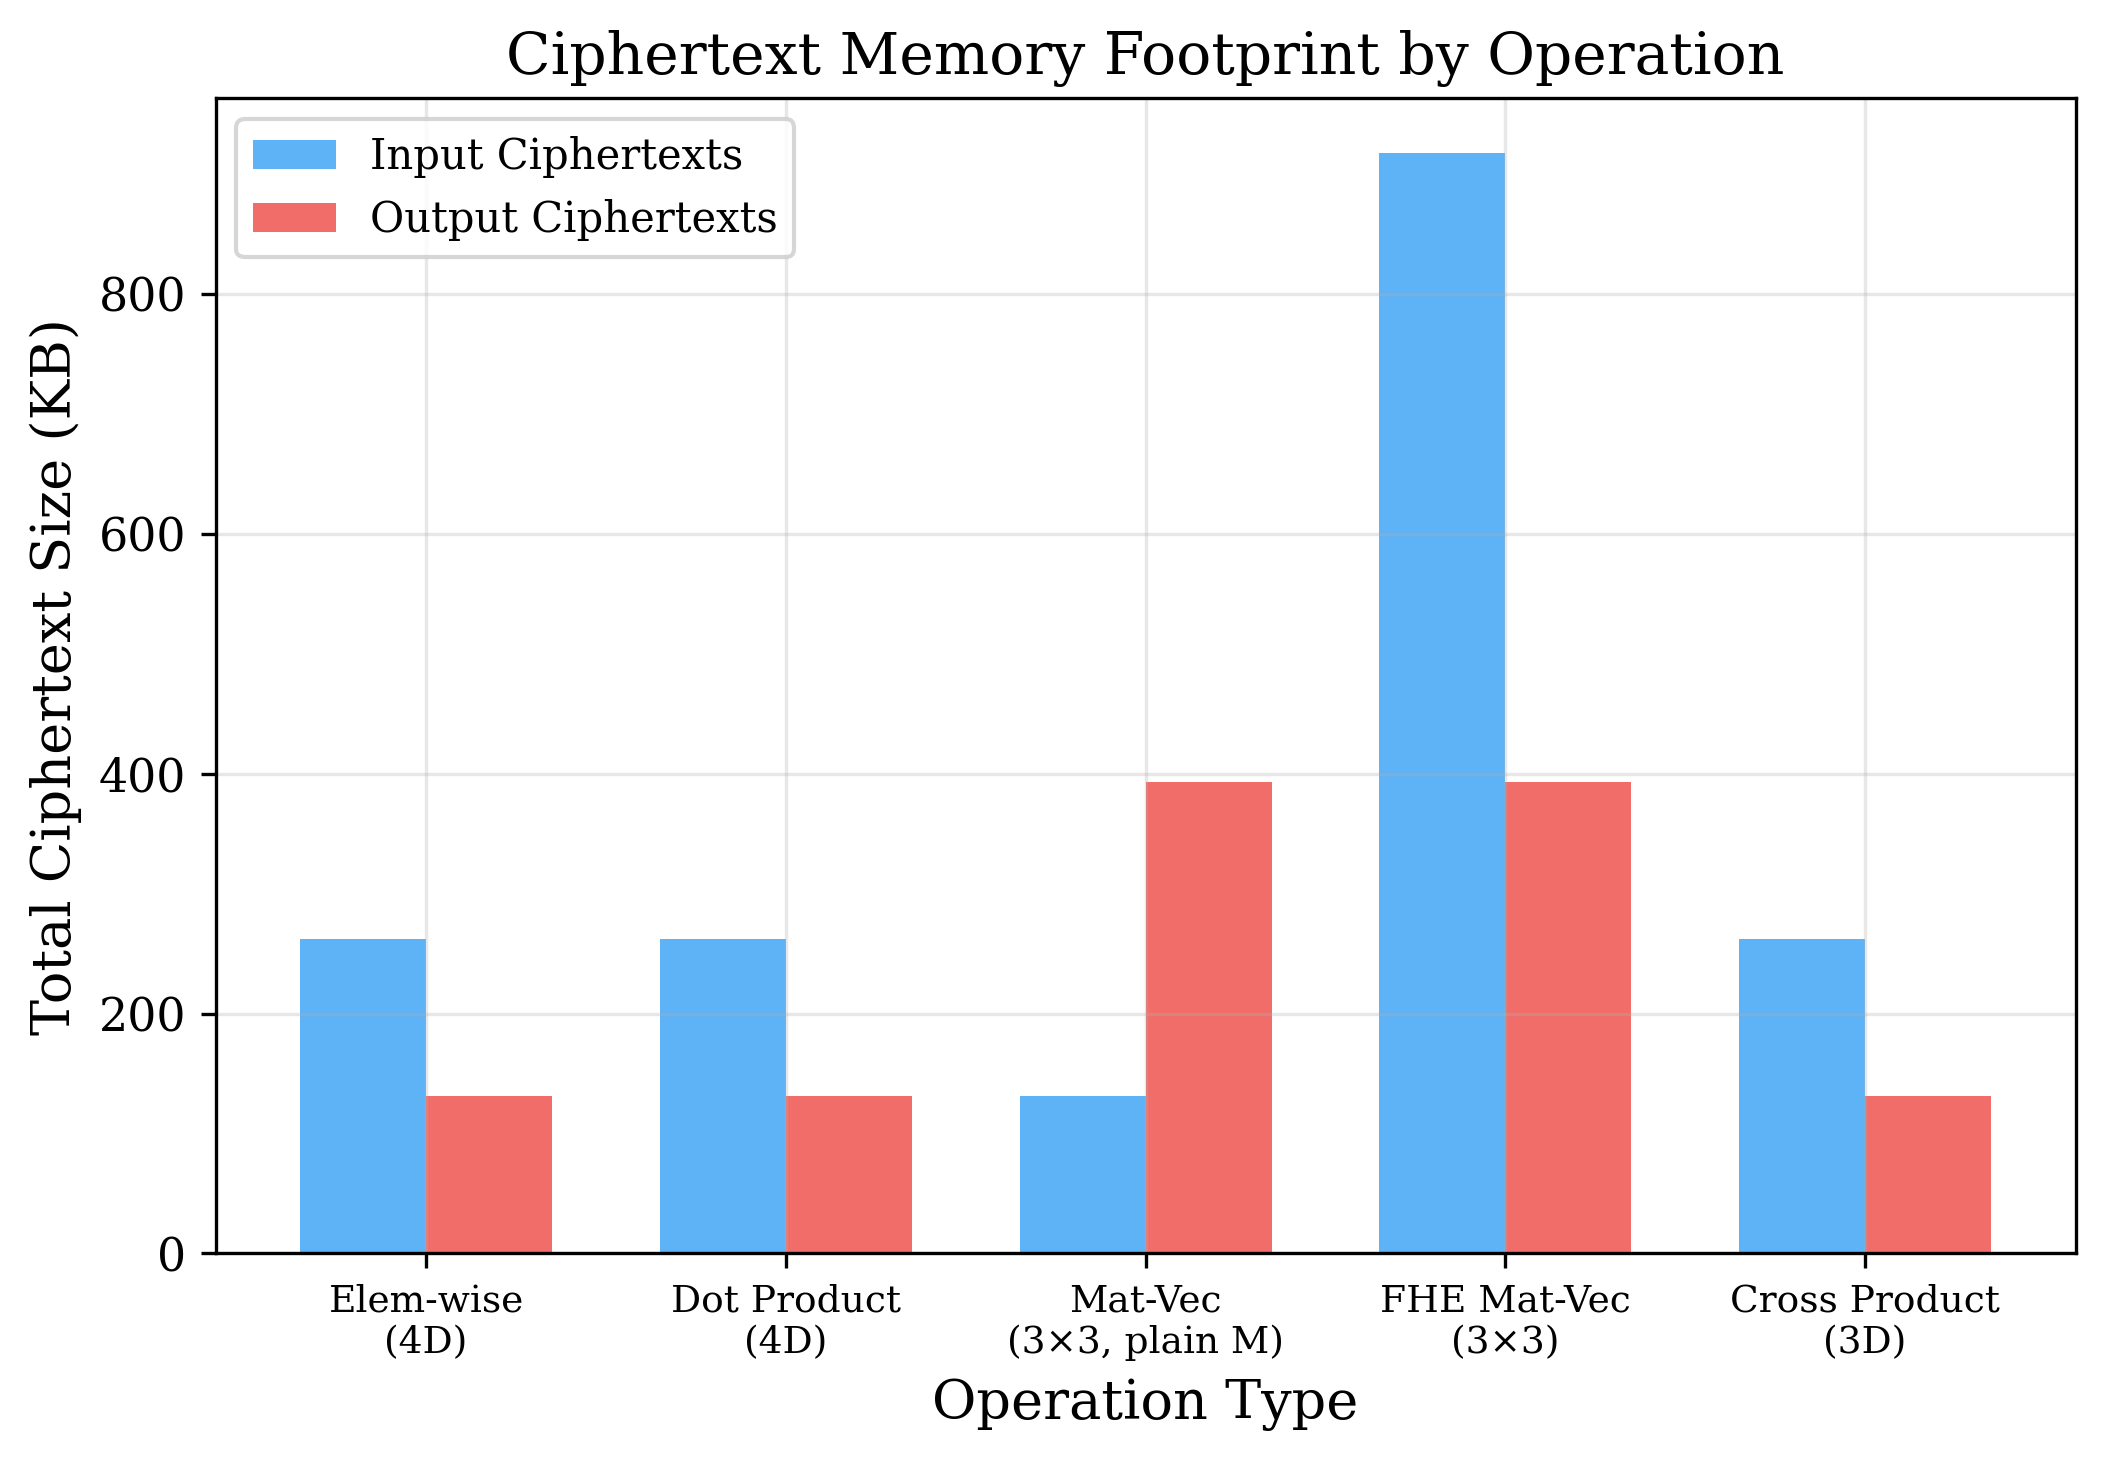
\includegraphics[width=\columnwidth]{fig_ciphertext_size.png}
    \caption{Ciphertext memory footprint comparison. FHE-MVM incurs $2m+1$ input ciphertexts vs.\ $m+1$ output ciphertexts.}
    \label{fig:ct_size}
\end{figure}

\FloatBarrier
\subsection{Scalability Analysis}

\begin{figure}[H]
    \centering
    
\includegraphics[width=\columnwidth]{fig_scalability.png}
    \caption{Scalability of encrypted demand aggregation. Overhead is $\sim$4000--5000$\times$ compared to plaintext, acceptable for 15-minute grid decision cycles.}
    \label{fig:scalability}
\end{figure}

\FloatBarrier
\subsection{ALT Accuracy Verification}

\begin{table}[H]
\centering
\caption{ALT Threshold Detection ($T{=}100$ kW, $k{=}7$)}
\label{tab:alt_accuracy}
\footnotesize
\resizebox{\columnwidth}{!}{%
\begin{tabular}{@{}ccccc@{}}
\toprule
\textbf{kW} & \textbf{True} & \textbf{Score} & \textbf{Zone} & \textbf{Conf.} \\
\midrule
50.0 & BELOW & $-0.25$ (clamp 0) & BELOW & 100\% \\
70.0 & BELOW & 0.050 & BELOW & 83\% \\
85.7 & BELOW & 0.000 & BELOW & 100\% \\
95.0 & BELOW & 0.325 & UNCERT. & 13\% \\
100.0 & AT & 0.500 & UNCERT. & 0\% \\
105.0 & ABOVE & 0.675 & UNCERT. & 13\% \\
114.3 & ABOVE & 1.000 & ABOVE & 100\% \\
130.0 & ABOVE & $1.75$ (clamp 1) & ABOVE & 100\% \\
\bottomrule
\end{tabular}}
\end{table}

\FloatBarrier
\subsection{Verification Protocol Testing}

\begin{table}[H]
\centering
\caption{Verifiable Aggregation Test Results}
\label{tab:ver_results}
\footnotesize
\resizebox{\columnwidth}{!}{%
\begin{tabular}{@{}lccp{3cm}@{}}
\toprule
\textbf{Scenario} & \textbf{Ag.} & \textbf{OK} & \textbf{Result} \\
\midrule
Honest coord. & 5 & \ding{51} & PASS \\
Honest coord. & 25 & \ding{51} & PASS \\
Inflated +10\,kW & 5 & \ding{55} & \textbf{DETECTED} \\
Deflated $-5$\,kW & 5 & \ding{55} & \textbf{DETECTED} \\
Agent excluded & 5 & \ding{55} & \textbf{DETECTED} \\
\bottomrule
\end{tabular}}
\end{table}

%==============================================================================
\section{Security Analysis}
\label{sec:security}
%==============================================================================

\subsection{CKKS Security}

The security of our system rests on the Ring Learning With Errors (RLWE) assumption. With $N = 16384$ and total coefficient modulus $\leq 438$ bits, the scheme achieves $\geq 128$-bit security per the Homomorphic Encryption Security Standard~\cite{HEStandard2018}. The public context (distributed to coordinator and agents) explicitly removes the secret key via \texttt{make\_context\_public()}, ensuring computational indistinguishability of ciphertexts.

\FloatBarrier
\subsection{Privacy Guarantees}

\begin{table}[H]
\centering
\caption{Privacy Guarantees by Operation}
\label{tab:privacy}
\footnotesize
\begin{tabular}{@{}lp{5cm}@{}}
\toprule
\textbf{Operation} & \textbf{Privacy Guarantee} \\
\midrule
Encryption & IND-CPA secure under RLWE \\
FHE-MVM & Both matrix \& vector encrypted \\
Dot product & Result encrypted; inputs hidden \\
ALT & Score encrypted; coord.\ sees $E(S)$ \\
Aggregation & Individual $d_i$ hidden in aggregate \\
Commitment & Perfectly hiding; reveals nothing \\
\bottomrule
\end{tabular}
\end{table}

\subsection{Integrity Verification}

Every \texttt{EncryptedDemand} object carries a SHA-256 checksum computed over the serialized ciphertext bytes. Before decryption, the utility verifies: $\text{SHA256}(\text{ct})_{[:12]} = \text{stored\_checksum}$. This detects any tampering with ciphertexts during transmission.

\subsection{Coordinator Honesty Enforcement}

The Pedersen commitment protocol ensures that any deviation by the coordinator (incorrect aggregation, agent exclusion, value manipulation) is detected with probability~1 by the utility's verification step. The soundness relies on the discrete logarithm assumption in the 2048-bit MODP group.

%==============================================================================
\section{Discussion and Future Work}
\label{sec:discussion}
%==============================================================================

\textbf{Limitations.} (1)~FHE-MVM requires $\mathcal{O}(mn)$ ciphertext multiplications, becoming expensive for large matrices. The $10 \times 10$ case already requires $\sim$410\,ms. (2)~Matrix rows are encoded as individual ciphertexts, limiting scalability due to per-ciphertext overhead. (3)~ALT provides soft classification only, not exact binary comparison. (4)~The cross product consumes 2 multiplicative levels, limiting subsequent operations. (5)~CKKS approximate decryption may leak information under adaptive attacks~\cite{Li2021ckks}; care must be taken with decryption results.

\textbf{Future Work.} (1)~Integrate CKKS bootstrapping~\cite{Cheon2018bootstrapping, Bossuat2021} for arbitrary-depth matrix operations. (2)~Block-packing strategies~\cite{Jiang2018} to encode multiple matrix rows per ciphertext, reducing communication. (3)~Extend to encrypted matrix--matrix multiplication for federated learning. (4)~Multiparty CKKS~\cite{Mouchet2020} to distribute key generation among households. (5)~GPU-accelerated CKKS for real-time large-scale grid analytics. (6)~Formal security proofs under the Universal Composability framework. (7)~Application to encrypted optimal power flow, state estimation, and demand forecasting with encrypted neural networks.

%==============================================================================
\section{Conclusion}
\label{sec:conclusion}
%==============================================================================

We have presented a comprehensive framework for secure linear algebra over CKKS-encrypted vectors, with the primary contribution being \textbf{fully homomorphic matrix--vector multiplication} (FHE-MVM) where both operands remain encrypted throughout computation. Our row-decomposition strategy decomposes the problem into $m$ encrypted dot products, each computed via SIMD element-wise multiplication and rotation-and-add summation, consuming only \textbf{one multiplicative level} regardless of matrix dimension. We additionally implemented encrypted element-wise multiplication, encrypted dot products, and encrypted cross products via permutation-matrix rotations.

Our system achieves 128-bit security with TenSEAL's CKKS implementation ($N=16384$, $\Delta=2^{40}$), demonstrating numerical errors within $10^{-7}$ relative tolerance for all operations except the depth-2 cross product ($10^{-4}$). The Adaptive Linear Threshold method achieves practical encrypted comparison with zero multiplicative depth, and the Pedersen commitment-based verifiable aggregation detects all coordinator misbehavior with probability~1. The interactive research dashboard provides unprecedented cryptographic transparency with ciphertext visualization, real-time profiling, and integrity verification.

%==============================================================================
\begin{thebibliography}{40}

\bibitem{Rivest1978}
R.~L.~Rivest, L.~Adleman, and M.~L.~Dertouzos, ``On data banks and privacy homomorphisms,'' in \emph{Foundations of Secure Computation}, 1978, pp.~169--180.

\bibitem{Gentry2009}
C.~Gentry, ``Fully homomorphic encryption using ideal lattices,'' in \emph{Proc.\ 41st ACM STOC}, 2009, pp.~169--178.

\bibitem{Brakerski2011}
Z.~Brakerski and V.~Vaikuntanathan, ``Efficient fully homomorphic encryption from (standard) LWE,'' in \emph{Proc.\ IEEE FOCS}, 2011, pp.~97--106.

\bibitem{Fan2012}
J.~Fan and F.~Vercauteren, ``Somewhat practical fully homomorphic encryption,'' \emph{IACR ePrint}, 2012/144, 2012.

\bibitem{Cheon2017}
J.~H.~Cheon, A.~Kim, M.~Kim, and Y.~Song, ``Homomorphic encryption for arithmetic of approximate numbers,'' in \emph{ASIACRYPT}, 2017, pp.~409--437.

\bibitem{Cheon2018bootstrapping}
J.~H.~Cheon, K.~Han, A.~Kim, M.~Kim, and Y.~Song, ``Bootstrapping for approximate homomorphic encryption,'' in \emph{EUROCRYPT}, 2018, pp.~360--384.

\bibitem{Paillier1999}
P.~Paillier, ``Public-key cryptosystems based on composite degree residuosity classes,'' in \emph{EUROCRYPT}, 1999, pp.~223--238.

\bibitem{Pedersen1991}
T.~P.~Pedersen, ``Non-interactive and information-theoretic secure verifiable secret sharing,'' in \emph{CRYPTO}, 1991, pp.~129--140.

\bibitem{McDaniel2009}
P.~McDaniel and S.~McLaughlin, ``Security and privacy challenges in the smart grid,'' \emph{IEEE Security \& Privacy}, vol.~7, no.~3, pp.~75--77, 2009.

\bibitem{Molina2010}
A.~Molina-Markham, P.~Shenoy, K.~Fu, E.~Cecchet, and D.~Irwin, ``Private memoirs of a smart meter,'' in \emph{ACM BuildSys}, 2010, pp.~61--66.

\bibitem{Lisovich2010}
M.~Lisovich, D.~Mulligan, and S.~Wicker, ``Inferring personal information from demand-response systems,'' \emph{IEEE Security \& Privacy}, vol.~8, no.~1, pp.~11--20, 2010.

\bibitem{Voigt2017}
P.~Voigt and A.~von dem Bussche, \emph{The EU General Data Protection Regulation (GDPR)}, Springer, 2017.

\bibitem{Li2010}
F.~Li, B.~Luo, and P.~Liu, ``Secure information aggregation for smart grids using homomorphic encryption,'' in \emph{IEEE SmartGridComm}, 2010, pp.~327--332.

\bibitem{Garcia2011}
F.~D.~Garcia and B.~Jacobs, ``Privacy-friendly energy-metering via homomorphic encryption,'' in \emph{STM}, 2011, pp.~226--238.

\bibitem{Erkin2012}
Z.~Erkin and G.~Tsudik, ``Private computation of spatial and temporal power consumption with smart meters,'' in \emph{ACNS}, 2012, pp.~561--577.

\bibitem{Lu2012}
R.~Lu, X.~Liang, X.~Li, X.~Lin, and X.~Shen, ``EPPA: An efficient and privacy-preserving aggregation scheme for secure smart grid communications,'' \emph{IEEE TPDS}, vol.~23, no.~9, pp.~1621--1631, 2012.

\bibitem{Acs2011}
G.~Acs and C.~Castelluccia, ``I have a DREAM! Differentially private smart metering,'' in \emph{ACM IH}, 2011, pp.~118--132.

\bibitem{Shi2011}
E.~Shi, T.-H.~H.~Chan, E.~Rieffel, R.~Chow, and D.~Song, ``Privacy-preserving aggregation of time-series data,'' in \emph{NDSS}, 2011.

\bibitem{Kursawe2011}
K.~Kursawe, G.~Danezis, and M.~Kohlweiss, ``Privacy-friendly aggregation for the smart-grid,'' in \emph{PETS}, 2011, pp.~175--191.

\bibitem{Bao2015}
H.~Bao and R.~Lu, ``A new differentially private data aggregation with fault tolerance for smart grid communications,'' \emph{IEEE IoT J.}, vol.~2, no.~3, pp.~248--258, 2015.

\bibitem{Guan2017}
Z.~Guan et al., ``Privacy-preserving and efficient aggregation based on blockchain for power grid communications,'' \emph{IEEE Commun.\ Mag.}, vol.~56, no.~7, pp.~82--88, 2018.

\bibitem{Aono2017}
Y.~Aono, T.~Hayashi, L.~Wang, S.~Moriai, et al., ``Privacy-preserving deep learning via additively homomorphic encryption,'' \emph{IEEE TIFS}, vol.~13, no.~5, pp.~1333--1345, 2017.

\bibitem{Takabi2016}
H.~Takabi, E.~Hesamifard, and M.~Ghasemi, ``Privacy preserving multi-party machine learning with homomorphic encryption,'' in \emph{NeurIPS PriML Workshop}, 2016.

\bibitem{Wood2019}
A.~Wood, K.~Najarian, and D.~Kahrobaei, ``Homomorphic encryption for machine learning in medicine and bioinformatics,'' \emph{ACM Comput.\ Surv.}, vol.~53, no.~4, pp.~1--35, 2020.

\bibitem{SEAL2022}
Microsoft Research, ``Microsoft SEAL (release 4.1),'' \url{https://github.com/Microsoft/SEAL}, 2022.

\bibitem{Halevi2014}
S.~Halevi and V.~Shoup, ``Algorithms in HElib,'' in \emph{CRYPTO}, 2014, pp.~554--571.

\bibitem{PALISADE2021}
PALISADE Lattice Cryptography Library, \url{https://palisade-crypto.org/}, 2021.

\bibitem{Benaissa2021}
A.~Benaissa, B.~Retiat, B.~Cebere, and A.~E.~Belfedhal, ``TenSEAL: A library for encrypted tensor operations using homomorphic encryption,'' \emph{ICLR DPML Workshop}, 2021.

\bibitem{Mouchet2020}
C.~Mouchet, J.~Troncoso-Pastoriza, J.-P.~Bossuat, and J.-P.~Hubaux, ``Multiparty homomorphic encryption from ring-learning-with-errors,'' \emph{PETS}, vol.~2021, no.~4, pp.~291--311, 2021.

\bibitem{OpenFHE2022}
A.~Al Badawi et al., ``OpenFHE: Open-source fully homomorphic encryption library,'' in \emph{ACM CCS WAHC}, 2022, pp.~53--63.

\bibitem{Chillotti2020}
I.~Chillotti, N.~Gama, M.~Georgieva, and M.~Izabach\`{e}ne, ``TFHE: Fast fully homomorphic encryption over the torus,'' \emph{J.\ Cryptology}, vol.~33, pp.~34--91, 2020.

\bibitem{Halevi2014matmul}
S.~Halevi and V.~Shoup, ``Bootstrapping for HElib,'' in \emph{EUROCRYPT}, 2015, pp.~641--670.

\bibitem{Juvekar2018}
C.~Juvekar, V.~Vaikuntanathan, and A.~Chandrakasan, ``GAZELLE: A low latency framework for secure neural network inference,'' in \emph{USENIX Security}, 2018, pp.~1651--1669.

\bibitem{CryptoNets2016}
R.~Gilad-Bachrach et al., ``CryptoNets: Applying neural networks to encrypted data with high throughput and accuracy,'' in \emph{ICML}, 2016, pp.~201--210.

\bibitem{Jiang2018}
X.~Jiang, M.~Kim, K.~Lauter, and Y.~Song, ``Secure outsourced matrix computation and application to neural networks,'' in \emph{ACM CCS}, 2018, pp.~1209--1222.

\bibitem{Kim2020}
A.~Kim, Y.~Song, M.~Kim, K.~Lee, and J.~H.~Cheon, ``Logistic regression model training based on the approximate homomorphic encryption,'' \emph{BMC Med.\ Genomics}, vol.~11, Suppl~4, 2018.

\bibitem{Boemer2019}
F.~Boemer, Y.~Lao, R.~Cammarota, and C.~Wierzynski, ``nGraph-HE: A graph compiler for deep learning on homomorphically encrypted data,'' in \emph{ACM CF}, 2019, pp.~3--13.

\bibitem{Dathathri2019}
R.~Dathathri et al., ``CHET: An optimizing compiler for fully-homomorphic neural-network inferencing,'' in \emph{ACM PLDI}, 2019, pp.~142--156.

\bibitem{Kim2018comparison}
M.~Kim, Y.~Song, and J.~H.~Cheon, ``Approximate homomorphic encryption over the conjugate-extended number fields,'' \emph{J.\ Math.\ Cryptol.}, 2019.

\bibitem{Cheon2019comparison}
J.~H.~Cheon, D.~Kim, and D.~Kim, ``Efficient homomorphic comparison methods with optimal complexity,'' in \emph{ASIACRYPT}, 2020, pp.~221--256.

\bibitem{Lu2021}
W.~Lu and J.~Zheng, ``Optimized comparison operations for CKKS,'' in \emph{CT-RSA}, 2021.

\bibitem{Iliashenko2021}
I.~Iliashenko and V.~Zucca, ``Faster homomorphic comparison operations for BGV and BFV,'' \emph{PETS}, vol.~2021, no.~3, 2021.

\bibitem{Lee2022}
E.~Lee et al., ``Low-complexity deep convolutional neural networks on fully homomorphic encryption using multiplexed parallel convolutions,'' in \emph{ICML}, 2022.

\bibitem{Gennaro2010}
R.~Gennaro, C.~Gentry, and B.~Parno, ``Non-interactive verifiable computing: Outsourcing computation to untrusted workers,'' in \emph{CRYPTO}, 2010, pp.~465--482.

\bibitem{Fiore2016}
D.~Fiore, R.~Gennaro, and V.~Pastro, ``Efficiently verifiable computation on encrypted data,'' in \emph{ACM CCS}, 2014, pp.~844--855.

\bibitem{Bultel2019}
X.~Bultel et al., ``Verifiable private multi-party computation: An application to smart grids,'' in \emph{ESORICS}, 2019.

\bibitem{Bayer2012}
S.~Bayer and J.~Groth, ``Efficient zero-knowledge argument for correctness of a shuffle,'' in \emph{EUROCRYPT}, 2012, pp.~263--280.

\bibitem{Boneh2019}
D.~Boneh, E.~Boyle, H.~Corrigan-Gibbs, N.~Gilboa, and Y.~Ishai, ``Zero-knowledge proofs on secret-shared data via fully linear PCPs,'' in \emph{CRYPTO}, 2019, pp.~67--97.

\bibitem{Costache2016}
A.~Costache and N.~P.~Smart, ``Which ring based somewhat homomorphic encryption scheme is best?'' in \emph{CT-RSA}, 2016, pp.~325--340.

\bibitem{Han2020}
K.~Han and D.~Ki, ``Better bootstrapping for approximate homomorphic encryption,'' in \emph{CT-RSA}, 2020, pp.~364--390.

\bibitem{Li2021ckks}
B.~Li and D.~Micciancio, ``On the security of homomorphic encryption on approximate numbers,'' in \emph{EUROCRYPT}, 2021, pp.~648--677.

\bibitem{Bossuat2021}
J.-P.~Bossuat, C.~Mouchet, J.~Troncoso-Pastoriza, and J.-P.~Hubaux, ``Efficient bootstrapping for approximate homomorphic encryption with non-sparse keys,'' in \emph{EUROCRYPT}, 2021, pp.~587--617.

\bibitem{Chen2019params}
H.~Chen, I.~Chillotti, and Y.~Song, ``Improved bootstrapping for approximate homomorphic encryption,'' in \emph{EUROCRYPT}, 2019, pp.~34--54.

\bibitem{HEStandard2018}
M.~Albrecht et al., ``Homomorphic encryption security standard,'' \emph{HomomorphicEncryption.org}, Toronto, Canada, 2018.

\end{thebibliography}

\end{document}
